
\documentclass[conference]{IEEEtran}

\usepackage[T1]{fontenc}
\usepackage{lmodern}
\usepackage{graphicx}
\usepackage{amsmath,amssymb}
\usepackage{booktabs}
\usepackage{hyperref}
\usepackage{xurl}
\usepackage{listings}
\usepackage{algorithm}
\usepackage{algpseudocode}

\hypersetup{
  colorlinks=true,
  linkcolor=blue,
  urlcolor=blue,
  citecolor=blue
}

\lstset{
  basicstyle=\ttfamily\footnotesize,
  columns=fullflexible,
  breaklines=true,
  frame=single,
  showstringspaces=false
}

\title{Pizzo: A Gamified Route-Planning Application Combining the Chinese Postman Problem and Blackjack Decision Support}

\author{
\IEEEauthorblockN{Tarik Agi\'c}
\IEEEauthorblockA{
Faculty of Electrical Engineering, University of Sarajevo\\
Sarajevo, Bosnia and Herzegovina\\
Student ID: 20108\\
Course: Artificial Intelligence
}
}

\begin{document}
\maketitle

\begin{abstract}
\emph{Pizzo} is an interactive desktop application that combines a graph-optimization task with a probabilistic decision-making mini-game.
In the narrative framing, ``pizzo'' refers to protection money collected by an Italian mafia capo.
If a city is modeled as a weighted, connected, undirected graph where intersections are vertices and streets are edges, then Toni must traverse the city to visit every business located along the streets.
To minimize fuel cost and exposure risk, Toni seeks the shortest closed walk that covers every street at least once---the \emph{Chinese Postman Problem} (CPP)~\cite{ref_mit_urban}.
After a long day of collecting pizzo, Toni relaxes by playing Blackjack (``21''), trying to increase his bankroll.
The Blackjack module includes an \emph{Advisor} (``Consigliere'') that computes the expected value (EV) of \textsc{Hit} versus \textsc{Stand} under an infinite-deck probability model, and recommends the statistically best action.
\end{abstract}

\begin{IEEEkeywords}
Chinese Postman Problem, graph optimization, Dijkstra's algorithm, minimum-weight perfect matching, Euler circuit, Blackjack, expectimax, expected value.
\end{IEEEkeywords}

\section{Introduction}
This project implements a single application with two tightly connected gameplay loops:
(1) a route-planning loop based on the Chinese Postman Problem (CPP) on an undirected weighted graph, and
(2) a Blackjack mini-game that shares the same bankroll as the route-planning loop.

The CPP portion models ``neighborhoods'' as weighted undirected graphs loaded from plain text files.
The user selects a neighborhood, chooses a start node by clicking a vertex, and the application computes and animates a CPP tour beginning at that vertex.
The animation includes a speed slider and a start/stop control, and the traversal updates the global wallet according to a reward/penalty formula implemented in the code.
The Blackjack portion is opened from the main window as a separate window; it provides a standard \textsc{Hit}/\textsc{Stand} flow with a dealer that hits until $\ge 17$, and it uses the same wallet and bet state as the main mode.

A key design goal was that every number shown in the GUI is computed from the underlying algorithmic state:
for example, the main HUD shows the sum of unique edge weights (original graph cost), the number of odd vertices, and the realized CPP tour cost (sum of step costs in the final walk).
These values correspond directly to fields computed in \texttt{MainView.h} and the CPP solver modules.

\section{Background and Problem Definitions}
\subsection{City as a Graph}
A neighborhood is modeled as an undirected connected graph $G=(V,E)$.
Each vertex $v\in V$ represents an intersection (or a point of interest), and each edge $e=(u,v)\in E$ represents a street segment connecting two intersections.
Each edge has a positive integer weight $w(u,v)$ representing traversal cost (distance).

In the implementation, the graph is stored as an adjacency list.
When an undirected edge is added, two directed adjacency entries are inserted (one for each direction), but they share a single unique edge identifier.
This shared identifier is crucial for Euler traversal because it allows each undirected edge to be marked ``used'' exactly once.

\subsection{Euler Circuits and Odd Vertices}
An \emph{Euler circuit} is a closed walk that uses every edge exactly once.
A connected undirected graph has an Euler circuit if and only if \emph{every vertex has even degree}~\cite{ref_euler_mathworld}.
Vertices of odd degree are central to CPP: if any vertex has odd degree, then no Euler circuit exists without duplicating some edges.
The CPP solution is therefore ``Eulerization'': duplicating a set of edges (or paths) so that all degrees become even, enabling an Euler circuit in an augmented multigraph.

\subsection{Chinese Postman Problem (CPP)}
The undirected CPP asks for the minimum-cost closed walk that traverses every edge at least once~\cite{ref_mit_urban}.
For undirected graphs, a classical solution pipeline is:
\begin{enumerate}
    \item Compute all odd-degree vertices.
    \item Compute shortest-path distances between all pairs of odd vertices.
    \item Find a minimum-weight perfect matching on the odd vertices using those distances.
    \item Duplicate the shortest paths for the matched pairs (augment the graph).
    \item Compute an Euler circuit in the augmented graph (e.g., Hierholzer's algorithm)~\cite{ref_hierholzer}.
\end{enumerate}
This project implements exactly that pipeline in \texttt{CPP.cpp} using \texttt{Dijkstra}, a brute-force minimum perfect matching routine, and a Hierholzer-style Euler circuit routine.

\subsection{Blackjack (``21'')}
Blackjack is a card game in which the player attempts to obtain a hand value as close to 21 as possible without exceeding it (busting).
Cards 2--10 have their face value, J/Q/K count as 10, and Ace can be 11 or 1 depending on what keeps the hand legal.
The player chooses \textsc{Hit} to draw another card or \textsc{Stand} to end drawing; then the dealer plays under deterministic rules (hit until $\ge 17$, stand otherwise), and the hands are compared.

In this project, Blackjack is simplified to the \textsc{Hit}/\textsc{Stand} action space with the dealer hitting until total $\ge 17$.
The Advisor computes the expected value of actions under an infinite-deck rank distribution (each rank is sampled with probability $1/13$).

\section{System Overview and Architecture}
\subsection{Modules}
The codebase is split into:
\begin{itemize}
    \item \textbf{Graph \& Algorithms (CPP):} \texttt{Graph}, \texttt{Dijkstra}, \texttt{Matching}, \texttt{Euler}, \texttt{CPP}, and \texttt{Route}.
    \item \textbf{Neighborhood I/O:} \texttt{Loader} and optional \texttt{NeighborhoodPicker}.
    \item \textbf{Blackjack Core:} \texttt{Card}, \texttt{Hand}, \texttt{BlackjackGame}, \texttt{Advisor}.
    \item \textbf{GUI:} \texttt{Application}, \texttt{MainWindow}/\texttt{MainView}, \texttt{BlackjackWindow}/\texttt{BlackjackView}, shared \texttt{GameState}, and \texttt{CommonTypes}.
\end{itemize}

\subsection{Shared State Between Modes}
The two modes share a global wallet and bet through \texttt{GameState.h}, implemented as \texttt{inline static} integers.
The wallet is updated both by the CPP traversal (rewards/penalties) and by Blackjack payouts.
This design makes the Blackjack mini-game meaningfully integrated rather than a separate demonstration.

\section{Neighborhood Data, Loading, and Automatic Visualization}
\subsection{Neighborhood File Format}
Neighborhood graphs are loaded from plain text files using \texttt{Loader}.
The format supported by the loader includes:
\begin{itemize}
  \item \texttt{V n}: number of vertices.
  \item \texttt{LABELS ...}: optional vertex labels (strings).
  \item \texttt{E u v cost}: an undirected weighted edge.
  \item Comment lines beginning with \texttt{\#} are ignored.
\end{itemize}

This format allows creating new neighborhoods without modifying the code: as long as a file describes $V$, optional labels, and edges, the loader will produce a graph, and the GUI will draw it.

\subsection{Provided Neighborhoods and Intended Variety}
The GUI exposes three neighborhood choices defined in \texttt{MainView.h}:
\textsc{Little Italy} (\texttt{neighborhood1.txt}),
\textsc{North Jersey} (\texttt{neighborhood2.txt}), and
\textsc{Pine Barrens} (\texttt{neighborhood3.txt}).
These three maps provide algorithmic variety:
\begin{itemize}
  \item \textbf{Little Italy} is small (6 vertices, 8 edges) and is useful for quickly visualizing the CPP pipeline.
  \item \textbf{North Jersey} is larger and denser (10 vertices, 19 edges), creating more route options and a more complex Eulerization effect.
  \item \textbf{Pine Barrens} is relatively sparse (8 vertices, 8 edges), illustrating how CPP handles lower connectivity while still requiring Eulerization when odd vertices exist.
\end{itemize}

Table~\ref{tab:neigh} summarizes the exact counts computed from the provided neighborhood text files.

\begin{table}[t]
\caption{Neighborhood Graph Statistics (from \texttt{neighborhood1--3.txt})}
\label{tab:neigh}
\centering
\begin{tabular}{lrrrr}
\toprule
Neighborhood & $|V|$ & $|E|$ & $\sum w(e)$ & \#odd \\
\midrule
Little Italy   & 6  & 8  & 32  & 4 \\
North Jersey   & 10 & 19 & 130 & 4 \\
Pine Barrens   & 8  & 8  & 40  & 4 \\
\bottomrule
\end{tabular}
\end{table}

\subsection{Automatic Node Layout in the GUI}
An automatic node-layout routine is implemented directly in the GUI.
After a neighborhood is loaded, the GUI computes positions for all vertices by placing them evenly on a circle:
for each vertex index $i\in\{0,\dots,N-1\}$, an angle
\[
  \theta_i = \frac{2\pi i}{N}
\]
is used, and the node is placed at
\[
  (x_i,y_i) = (x_c + R\cos\theta_i,\; y_c - R\sin\theta_i),
\]
where $(x_c,y_c)$ is the graph-rectangle center and $R$ is a radius chosen from the available panel size.
This matches the implemented loop in \texttt{MainView.h} which computes \texttt{ang}, \texttt{cos}, \texttt{sin}, and rounds the results to pixel coordinates.

Therefore, to add a new neighborhood, one only needs to add a new text file following the loader format and add a corresponding button entry; the drawing is automatic because it depends only on $N$ and the view rectangle.

\section{Chinese Postman Problem: Algorithm and Implementation}
\subsection{Pipeline Implemented in \texttt{CPP.cpp}}
The core CPP routine follows the classical undirected CPP method.
At a high level:

\begin{algorithm}[t]
\caption{Undirected Chinese Postman as Implemented}
\label{alg:cpp}
\begin{algorithmic}[1]
\Require Connected undirected weighted graph $G=(V,E)$, start vertex $s$
\Ensure Minimum-cost closed walk starting at $s$ that covers all edges
\State $O \gets \{v \in V \mid \deg(v)\ \text{is odd}\}$
\If{$O = \emptyset$}
  \State return EulerCircuit$(G,s)$
\EndIf
\State For each $o_i \in O$: run Dijkstra$(G,o_i)$ to get distances to all $o_j\in O$
\State Build distance matrix $D[i,j] = \text{dist}(o_i,o_j)$
\State $M \gets$ MinPerfectMatching$(O,D)$
\State $G' \gets G$ \Comment{copy as multigraph}
\ForAll{pairs $(o_i,o_j)\in M$}
  \State $P \gets$ reconstruct shortest vertex path from $o_i$ to $o_j$
  \State duplicate each edge along $P$ into $G'$
\EndFor
\State $C \gets$ EulerCircuit$(G',s)$
\State Convert consecutive vertices of $C$ into route steps and return
\end{algorithmic}
\end{algorithm}

The remainder of this section ties each pipeline step to a specific module and clarifies how cost is computed.

\subsection{Graph Representation and Edge Identifiers}
\texttt{Graph} stores adjacency lists, and each undirected edge is represented by two directed adjacency entries that share the same edge ID.
Euler traversal uses a boolean array \texttt{used[edgeId]} so an undirected edge is consumed exactly once, even though it appears twice in adjacency.

This is essential for Hierholzer traversal in undirected graphs: when the algorithm selects one directed adjacency entry, it marks the underlying undirected edge as used and will skip the opposite direction later.

\subsection{Odd Vertices and Why They Matter}
If the graph is not Eulerian, the number of odd-degree vertices is even.
The CPP solution adds (duplicates) edges so that odd vertices become even, enabling an Euler circuit.
In the GUI, the number of odd vertices is computed from the loaded graph and displayed in the HUD (e.g., ``Odd Vertices: 4'').

\subsection{Shortest Paths Between Odd Vertices (Dijkstra)}
To decide which edges to duplicate, the solver requires the shortest-path distances between odd vertices.
The project implements Dijkstra's algorithm over the adjacency list.
For each odd vertex $o_i$, Dijkstra computes distances to all vertices and stores a parent pointer array, which later enables reconstruction of an explicit path between matched vertices.

\subsection{Minimum Perfect Matching of Odd Vertices}
The solver forms pairs of odd vertices such that the sum of distances between paired vertices is minimized.
This is a minimum-weight perfect matching problem on the complete graph induced by odd vertices, with edge weights equal to shortest-path distances.

In this codebase, \texttt{Matching.cpp} implements a brute-force recursive pairing strategy:
it picks the first unpaired odd vertex, tries pairing it with every other unpaired odd vertex, and recurses to complete the matching, keeping the minimal total cost.
This approach is exact for small numbers of odd vertices and matches the intended scale of the provided neighborhoods (each has exactly four odd vertices, i.e., only three possible matchings).

\subsection{Eulerization by Duplicating Shortest Paths}
For each pair $(o_i,o_j)$ in the matching, the solver reconstructs the shortest vertex path in the original graph and duplicates each edge along that path into an augmented graph $G'$.
Because the augmented graph is a multigraph, duplicating edges increases degrees appropriately without deleting original edges.

\subsection{Euler Circuit via Hierholzer-Style Traversal}
Once $G'$ is Eulerian (all degrees even), the solver computes an Euler circuit beginning at the selected start node.
The implementation in \texttt{Euler.cpp} is a Hierholzer-style algorithm and includes a correctness check that the circuit length is $|E'|+1$; otherwise, it throws an error indicating a disconnected graph (no valid Euler circuit).

\subsection{Cost Accounting in the HUD}
The main view displays three key quantities:
\begin{itemize}
  \item \textbf{Sum of Edges:} the sum of weights of all original edges counted once (unique edge cost).
  \item \textbf{Odd Vertices:} the number of odd-degree vertices in the original graph.
  \item \textbf{Real Path Cost:} the total cost of the computed CPP route, defined as the sum of costs of the step sequence produced from the Euler circuit in the augmented graph.
\end{itemize}

The CPP solver explicitly returns:
\begin{itemize}
  \item \texttt{originalCost}: the original unique edge sum.
  \item \texttt{addedCost}: the extra cost introduced by duplicating shortest paths for the matching.
  \item \texttt{totalCost}: \texttt{originalCost + addedCost}.
\end{itemize}
The GUI additionally computes the realized route cost from the produced step list.

\subsection{Representative Code Excerpt (CPP orchestration)}
The following excerpt illustrates that the solver (i) finds odd vertices, (ii) runs Dijkstra among odd vertices, (iii) matches them, (iv) augments the graph, and (v) computes Euler:
\begin{lstlisting}[language=C++]
auto odd = findOddVertices(g);
if (odd.empty()) {
  res.eulerCircuit = Euler::eulerCircuit(g, start);
  return res;
}
auto dist = buildOddDistanceMatrix(g, odd); // via Dijkstra
auto mr = Matching::minPerfectMatching(odd, dist);
Graph aug = g;
augmentByMatchedPaths(aug, g, odd, mr.pairs); // duplicate shortest paths
res.eulerCircuit = Euler::eulerCircuit(aug, start);
\end{lstlisting}
(Names are simplified for readability; this excerpt corresponds to the concrete control flow in \texttt{CPP.cpp}.)

\section{Gamification: Money Collection Logic During Traversal}
\subsection{Global Wallet}
The wallet is stored in \texttt{GameState::Wallet} and is shared across both game modes.
The CPP traversal updates the wallet each time the animated agent completes a route step.

\subsection{Per-Edge Reward and Per-Step Penalty}
The money logic is implemented in \texttt{MainView.h} with three constants:
\texttt{BASE\_REWARD = 40}, \texttt{WEIGHT\_BONUS = 10}, and \texttt{PENALTY = 3}.
Let $w$ be the integer weight of the traversed edge.
Then:
\begin{itemize}
  \item The first time an undirected edge is traversed, the wallet increases by
  \[
    \Delta^+ = 40 + 10\cdot w.
  \]
  \item Every traversal (including the first) decreases the wallet by
  \[
    \Delta^- = 3\cdot w.
  \]
\end{itemize}
Therefore, the \emph{net} change on first traversal of an edge is $(40 + 10w) - 3w = 40 + 7w$, while revisiting an edge yields a net change of $-3w$.

To ensure ``first time'' is defined per \emph{undirected} edge, the GUI tracks a set of rewarded edges keyed by the unordered pair $\{u,v\}$.
This design reinforces the CPP objective: duplicated edges (required when odd vertices exist) impose additional penalties during traversal.

\subsection{Traversal Speed Control}
The traversal is driven by a GUI timer constructed with a period of \texttt{0.04f} seconds.
Each tick advances the interpolation parameter by an animation speed derived from a slider.
The speed is mapped linearly between \texttt{\_animSpeedMin = 0.02f} and \texttt{\_animSpeedMax = 0.18f}.
Thus the GUI provides fine-grained control over how quickly the agent moves along route steps.

\section{Blackjack Module: Rules and Implementation}
\subsection{Card and Hand Representation}
Cards are represented by rank and suit.
For game logic, the hand value is computed from ranks:
2--9 map to their numeric values, 10/J/Q/K map to 10, and Ace initially maps to 11.
The \texttt{Hand} class tracks a running total and a boolean \texttt{soft} indicator.
When adding a card would cause the total to exceed 21 and \texttt{soft} is true, the total is reduced by 10 and \texttt{soft} is set false, effectively converting one Ace from 11 to 1.

\subsection{Round Flow}
The Blackjack game state:
\begin{itemize}
  \item Deals two cards to the player and two cards to the dealer at round start.
  \item Exposes two actions: \textsc{Hit} (draw one card) and \textsc{Stand} (end drawing).
  \item Implements the dealer policy: hit while dealer total $< 17$; otherwise stand.
\end{itemize}

\subsection{Betting and Payout}
The GUI uses \texttt{GameState::CurrentBet} and clamps it to the wallet.
At round start, the bet amount is subtracted from the wallet.
At round end, the payout is applied once:
\begin{itemize}
  \item Win (player wins or dealer busts): add $2\times$ bet (restoring stake plus winnings).
  \item Tie: add $1\times$ bet (stake returned).
  \item Loss: no addition (stake already removed).
\end{itemize}

\section{Advisor (Consigliere): Expected-Value Decision Support}
\subsection{Probability Model}
The Advisor assumes an infinite deck with uniform rank probability.
Each of the 13 ranks is drawn with probability $1/13$; consequently, the total probability of drawing a 10-valued card is $4/13$ (Ten, Jack, Queen, King).

\subsection{Dealer Outcome Distribution}
Given a dealer upcard rank, the Advisor computes a distribution over dealer terminal outcomes (bust or totals 17--21) by enumerating all possible hole-card ranks and recursively simulating the dealer policy (hit until $\ge 17$).
This recursion is memoized over dealer states \texttt{(total, soft)}.

\subsection{Player Expected Value}
Given the player's current state \texttt{(total, soft)} and the dealer upcard, the Advisor computes:
\begin{itemize}
  \item $\mathrm{EV}(\textsc{Stand})$: compare player total against the dealer distribution and assign payoff $+1$ for win, $0$ for tie, $-1$ for loss.
  \item $\mathrm{EV}(\textsc{Hit})$: enumerate each next card rank with probability $1/13$, update the player's state, and then evaluate the best achievable EV from that new state.
\end{itemize}
The continuation value after a hit is computed as:
\[
  \mathrm{EV}(s) = \max\{\mathrm{EV}(\textsc{Hit}\mid s),\ \mathrm{EV}(\textsc{Stand}\mid s)\},
\]
which is an expectimax-style optimal policy evaluation for a stochastic environment.

The Advisor memoizes player states by \texttt{(total, soft, dealerUp)} to ensure responsiveness in the GUI.
Finally, it recommends \textsc{Hit} if $\mathrm{EV}(\textsc{Hit}) > \mathrm{EV}(\textsc{Stand})$ and \textsc{Stand} otherwise, and displays both EV values in the advisor tooltip.

\section{Graphical User Interface and Features}
\subsection{Main Window (CPP Mode)}
The main window, titled \texttt{Pizzo}, contains:
\begin{itemize}
  \item A HUD with a play/pause button, traversal speed slider, and money display.
  \item A graph panel that renders the neighborhood graph and the computed tour.
  \item A neighborhood-selection panel with three provided neighborhood options.
  \item A \texttt{Blackjack} button that opens the Blackjack window.
\end{itemize}
The user selects a neighborhood, then clicks a node to begin; the HUD text indicates this state (``Select a node to begin'').

\subsection{Blackjack Window}
The Blackjack window renders:
\begin{itemize}
  \item The dealer hand (including a face-down card during play) and the player hand.
  \item \textsc{Hit} and \textsc{Stand} action buttons.
  \item A bankroll and bet control panel (increment/decrement buttons).
  \item A back button to close the window and return to the main mode.
\end{itemize}

\section{Conclusion}
\emph{Pizzo} demonstrates an end-to-end application that connects deterministic graph optimization (CPP) with stochastic decision-making (Blackjack).
The CPP mode implements the classical undirected CPP pipeline using Dijkstra shortest paths, minimum perfect matching of odd vertices, graph Eulerization, and a Hierholzer-style Euler circuit routine.
The Blackjack mode provides a playable mini-game that shares a wallet with the CPP traversal and includes a mathematically grounded EV-based Advisor.
Together, the system illustrates core algorithmic concepts (odd vertices, Euler circuits, shortest paths, matchings) and AI concepts (expectimax-style evaluation under chance) within a cohesive interactive narrative.

\bibliographystyle{IEEEtran}
\begin{thebibliography}{1}

\bibitem{ref_mit_urban}
MIT, \emph{Urban Operations Research}, ``Section 6.4.2.'' [Online]. Available: \url{https://web.mit.edu/urban_or_book/www/book/chapter6/6.4.2.html}. Accessed: 2026-02-16.

\bibitem{ref_euler_mathworld}
Wolfram MathWorld, ``Eulerian cycle.'' [Online]. Available: \url{https://mathworld.wolfram.com/EulerianCycle.html}. Accessed: 2026-02-16.

\bibitem{ref_hierholzer}
TUM Algorithms, ``Hierholzer's algorithm.'' [Online]. Available: \url{https://algorithms.discrete.ma.tum.de/graph-algorithms/hierholzer/index_en.html#}. Accessed: 2026-02-16.

\end{thebibliography}

\appendix
\section{Application Screenshots}

Figures~\ref{fig:main} and~\ref{fig:bj} show the two main application modes.

\begin{figure*}[t]
\centering
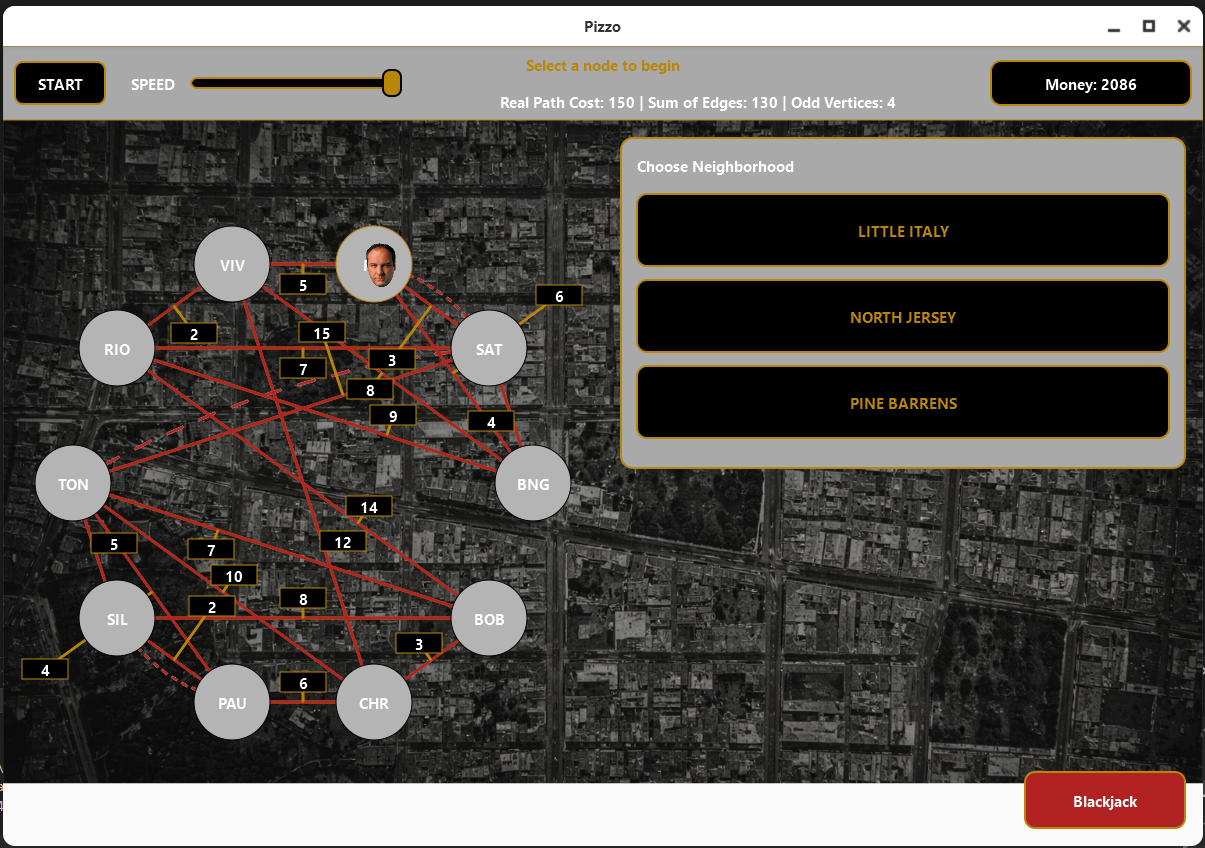
\includegraphics[width=0.95\textwidth]{Images/cpp.png}
\caption{Main mode (CPP): neighborhood selection, graph visualization, route statistics, speed control, and shared money display.}
\label{fig:main}
\end{figure*}

\begin{figure*}[t]
\centering
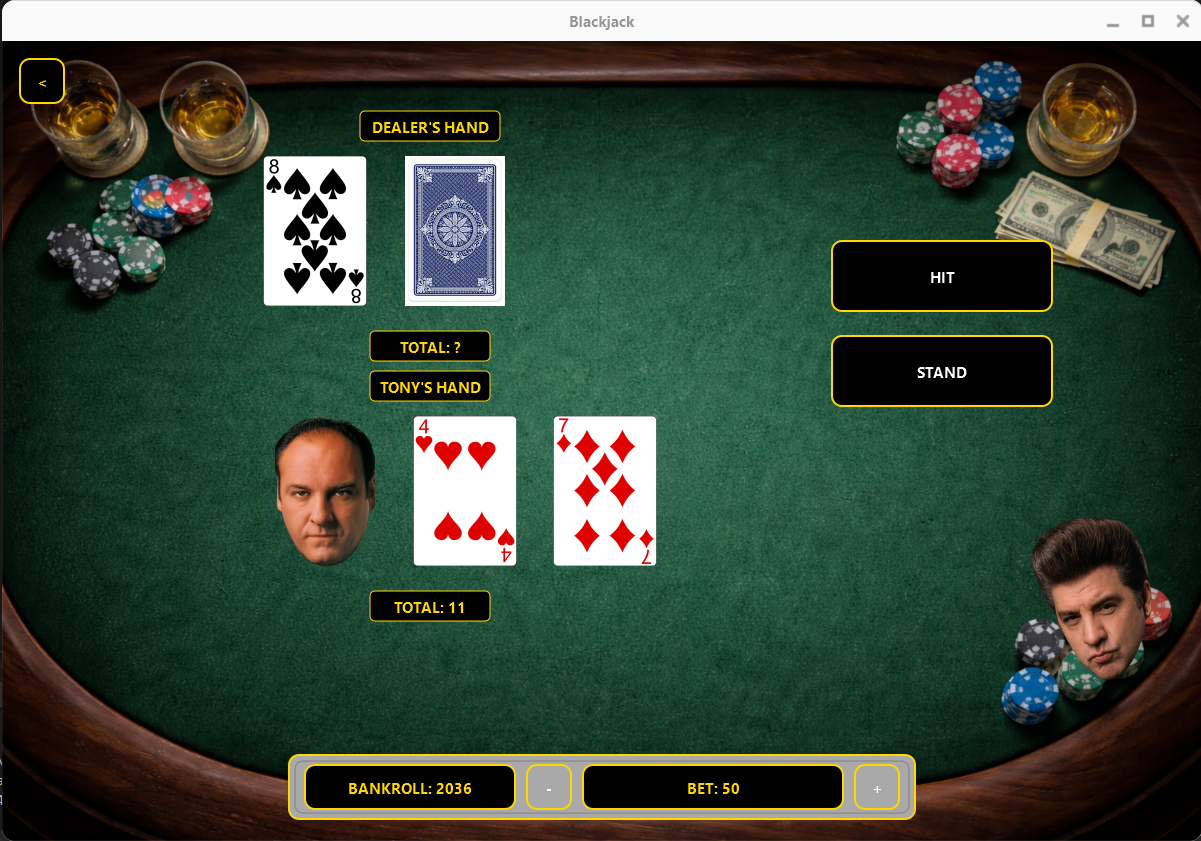
\includegraphics[width=0.95\textwidth]{Images/blackjack.png}
\caption{Blackjack mode: dealer and player hands, \textsc{Hit}/\textsc{Stand} actions, bankroll and bet controls, and integration with shared wallet.}
\label{fig:bj}
\end{figure*}

\end{document}